

\setcounter{chapter}{0}
\chapter*{Introduction}
\addcontentsline{toc}{chapter}{Introduction} %\markboth{INTRODUCTION}{}

``\textit{Change}, \textit{alter}, or perhaps \textit{transform}?'' Selecting the perfect word for a specific context, such as when composing a report or a speech, is all the easier with a thesaurus at hand. These lexicographic resources are invaluable for looking up alternative words or phrases that convey a specific meaning. Indeed, thesauri are sometimes included as course material to acquire a language as well as the nuances available within one.\footnote{See, for instance, Gánem-Gutiérrez and Gilmore, `A Mixed Methods Case Study on the Use and Impact of Web-based Lexicographic Tools on L2 Writing'. The authors state that thesauri, and other Web-based lexicographic resources, ``have become widely used by second language (L2) learners, particularly for academic writing'' (p. 1). Celen and Yalçin demonstrate benefits of such use in their article `The Effects of Vocabulary Resource Use on Lexical Richness in L2 Writing'. Turkish students' consulting of a thesaurus ``led to a significant increase in lexical sophistication'' in their English essays (p. 1039).} In addition, thesauri offer a number of uses beyond looking up alternative phrasings: they are veritable treasure troves for cultural, linguistic, anthropological, and literary-critical research --- especially when these resources are arranged in a topical fashion, a hierarchical ordering of its groups of loosely synonymous words according to their meaning.\footnote{Brewer, Review of \textit{Historical Thesaurus of the Oxford English Dictionary}, p. 802; Adamska-Salaciak, Review of \textit{Historical Thesaurus of the Oxford English Dictionary}, p. 232; Busse, `A Celebration of Words and Ideas', p. 88.} These topical thesauri -- or, more specifically, ones that cover a historical language -- take centre stage in this dissertation, which examines how their dissemination on the Web can be improved to facilitate research.

This introduction is organized as follows. Section \ref{sect:Introduction:Thesaurus} introduces the main topic of my dissertation, i.e., thesauri, more specifically, thesauri of historical languages. Next, section \ref{sect:Introduction:ThesaurusUses} offers an overview of the various research applications of a thesaurus. Section \ref{sect:Introduction:Impediments} discusses opportunities for improvement of the dissemination of these resources to this end. In section \ref{sect:Introduction:Objectives}, the research objective and questions can be found, followed by an outline of the dissertation in section \ref{sect:Introduction:Methodology}. Lastly, section \ref{sect:Introduction:Related} provides an overview of related work.



\section{Thesauri and historical languages}
\label{sect:Introduction:Thesaurus}

Historically, the term \textit{thesaurus} has been applied to a range of resources. The term, derived from Greek \textit{thēsauros} (``store, treasure''),\footnote{\textit{Oxford English Dictionary}, 2nd edn, s.v. `thesaurus, n.'.} has been used in the sense of a `classical lexicon', a `semantically organized dictionary', and a `terminological database' or `index'.\footnote{Hartmann, \textit{Encyclopedia of Language \& Linguistics}, s.v. `Thesauruses'} The first sense is now largely obsolete;\footnote{An example of a thesaurus in the sense of a classical lexicon is the \textit{Thesaurus Linguae Latinae}, an authoritative dictionary of ancient Latin that, according to the introduction provided on its website, covers ``all surviving Latin texts from the earliest times down to AD 600''.} the second and third, developed through semantic narrowing, are still current and, as will become apparent in the dissertation, are closely related to one another.\footnote{See Chapter 3.} The dissertation concentrates on the second meaning of the term,\footnote{In articles that demand distinguishing between the second and third sense, I apply the terms \textit{topical thesaurus} and \textit{indexing thesaurus}, respectively. Examples of the latter are the `NASA Thesaurus', `EuroVoc', and the `Medical Subject Headings RDF'.} which has been defined more specifically as ``a work of lexicographical reference which presents lexical facts with semantic domains as its core organizational principle, rather than in alphabetical arrangement''.\footnote{Kay and Alexander, `Diachronic and Synchronic Thesauruses', p. 367.}

The first semantically organized dictionary, published in 1852, was Peter Mark Roget's \textit{Thesaurus of English Words and Phrases} (henceforth \textit{Roget's}). This work by Roget (1779-1869), a British physician and theologian, was the first of its kind to arrange a lexicon -- that of contemporary English -- in groups of loosely synonymous words according to an overarching, hierarchical structure.\footnote{Hüllen, \textit{A History of Roget's} Thesaurus, p. 234.} This macrostructure can be likened to the taxonomies of animals and plants by Carl Linnaeus (1707-1778). In fact, Roget may even have taken these taxonomies of the natural kingdom as examples for his own structure.\footnote{Ibid., p. 18.} In these tree-like structures, the most generic or abstract concepts are used as roots, which branch out to groups of words increasingly specific in meaning.\footnote{Onomasiological approaches to language, which adopt a thematic arrangement of words and phrases rather than an alphabetical one, have a long history predating \textit{Roget's}. Early works of this kind, albeit not capturing the lexicon of an entire language, date back as far as Antiquity and possibly further still (Hüllen, \textit{A History of Roget's} Thesaurus, p. 44).} From the start, \textit{Roget's} was commercially successful and has remained popular to the present day --- with a distribution ``almost comparable to that of the Bible''.\footnote{Ibid., p. 1.}

Since the publication of \textit{Roget's}, a small number of thesauri have been fashioned that capture the lexicon belonging to a historical period rather than a contemporary one.\footnote{See Chapter 1.} Amongst these (though not the first) is \textit{A Thesaurus of Old English} (\textit{TOE}). \textit{TOE}, first published in 1995, is concerned with the Old English lexicon, the variant of English spoken between roughly 500 and 1100 by the Anglo-Saxons. This thesaurus has been met with high praise by scholars. Rolf H. Bremmer Jr, for instance, states that the thesaurus fills a ``voluminous gap [...] on the shelf of lexicographical tools'' available for Old English.\footnote{Bremmer, `Treasure Digging', p. 109.} Richard Dance, too, calls \textit{TOE} ``invaluable'' for lexical studies and deems it an ``impressive piece of scholarship''.\footnote{Dance, Review of \textit{A Thesaurus of Old English}, p. 312.} Manfred Görlach goes so far as to state that \textit{TOE} is ``the most important contribution to Old English studies for years'', since its ``comprehensive analysis'' allows scholars to ``investigate what distinctions Anglo-Saxons felt important enough to make in the lexicon''.\footnote{Görlach, Review of \textit{A Thesaurus of Old English}, pp. 398-9.} Like \textit{Roget's}, \textit{TOE} treats its lexicon as a temporally indistinguishable whole. Such thesauri are called synchronic. A diachronic one, charting the changes throughout a certain period, did not yet exist of an entire language when \textit{TOE} was published. However, \textit{TOE} was intended as a pilot of such a thesaurus.\footnote{Roberts, `\textit{A Thesaurus of Old English}: The Pilot Study for the Glasgow \textit{Historical Thesaurus}'.}

The first diachronic thesaurus of an entire language was published in 2009: \textit{The Historical Thesaurus of English} (\textit{HTE}).\footnote{Information on its versions can be found in the section `Versions of the Thesaurus'. The first version of this thesaurus was published as \textit{Historical Thesaurus of the Oxford English Dictionary}, and its contents are still available digitally on the website of the \textit{Oxford English Dictionary}. Although this thesaurus is the first diachronic one of an entire language, thesauri acting as pilots and foretastes have been published at earlier points in time. See \textit{TOE} and Coleman, \textit{Love, Sex and Marriage}.} This thesaurus charts the development of the entire English lexicon, from the Old English period up to the present. Its information on the Old English period came from \textit{TOE}; information from later periods was taken from the \textit{Oxford English Dictionary}. The annotation added for lexical items on period of use allows these items to be ordered not just by their meaning but also chronologically.\footnote{The dissertation adopts the term \textit{lexical item} to refer to a word or phrase in a single sense or across all of its senses. As such, \textit{lexical item} is a hypernym of \textit{lexical sense} and \textit{lexical entry} as defined in Lemon-OntoLex (`Lexicon Model for Ontologies), which, in turn, correspond with \textit{lexical unit} and \textit{lexeme} as defined by Cruse in \textit{Lexical Semantics}.} This diachronic approach for the English language as a whole allows for comprehensive investigations into semantic change.\footnote{Brewer, Review of \textit{Historical Thesaurus of the Oxford English Dictionary}, p. 802.} Additionally, the thesaurus allows for a focus on the vocabulary available in a specific time frame, such as that available to Shakespeare,\footnote{Kay et al., `Unlocking the OED', p. xiv.} providing the opportunity for more thorough investigations of historical stylistics. Owing to the new paths opened up to them, researchers have dubbed the thesaurus ``invaluable'' or even a ``godsend'', underlining the importance of such semantically organized dictionaries.\footnote{Coleman, Review of \textit{Historical Thesaurus of the Oxford English Dictionary}, p. 208; and Busse, `A Celebration of Words and Ideas', p. 88., respectively.}


\section{Thesauri and their applications}
\label{sect:Introduction:ThesaurusUses}

% Knowledge catalogued by onomasiological works have had numerous uses: interpretation of texts in foreign languages, selection of words or phrases more suitable in textual composition, and studies of entire semantic fields (Hüllen, 1999).30 

In addition to providing the means to locate and select available alternative phrasings, thesauri offer a number of applications valuable for research into language and culture. To illustrate, thesauri facilitate analyses and comparisons of semantic fields: groups of words related in meaning. Since lexical items located near each other in a topical thesaurus are by definition related in meaning, the words that make up a semantic field (e.g., for emotions) can more easily be pinpointed and subsequently scrutinized.\footnote{Diller, `Emotions in the English Lexicon'.} Moreover, when a thesaurus contains indications of the time frames in which words were used for specific meanings, the thesaurus can be used to research the development of the language it deals with.\footnote{Crystal, \textit{Words in Time and Place}.} To give an example, the word \textit{knight} has gained a meaning during the Middle English period that is more positive than in the preceding period: it used to denote simply `boy, youth attendant'. Such a semantic shift is known as amelioration. The opposite of amelioration is possible as well, called pejoration. An example of this semantic shift can be found with the lexical item \textit{knave}, meaning `crook', which was used to indicate the more neutral meaning of `boy, servant' in the Old English period.\footnote{For an introduction to amelioration and pejoration, including the examples mentioned here, see Schendl, \textit{Historical Linguistics}, p. 31.} Although such changes in meaning of lexical items may be discoverable through a historical dictionary, such as the \textit{Oxford English Dictionary}, too, a diachronic thesaurus offers the means to track these changes through the semantic framework constituted by its topical systems.\footnote{E.g., Kay and Wotherspoon, `Wreak, Wrack, Rack, and (W)ruin'.} Thus, gaps in meaning that such language changes came to fill in a lexicon can be traced across semantic fields. The same is true for gaps left behind by such changes. Competition between words and phrases within a semantic field is more apparent, too, by identifying and contrasting lexical items in a field that have survived or were newly coined with others in that field that disappeared from use.\footnote{E.g., Tejada-Caller, `On \textit{Shapelings} and \textit{Childlings}'.} Tracing developments in the language in such a manner is only one of the possible research uses for topical thesauri.


Another use for these lexicographic resources lies in research on metaphors.\footnote{Allan, \textit{Metaphor and Metonymy}.} By mapping out which words, or lexical items, can be used metaphorically to indicate other notions, it is possible to see which semantic fields in a language have close conceptual ties. As an example, words related to sleeping are not uncommonly used to indicate death, the everlasting sleep, as it were. Additionally, lexical items indicating temperature have a strong metaphorical link with those of emotions; a hot-headed person is one who is easily angered.\footnote{For both metaphorical ties mentioned, see \textit{Mapping Metaphor}.} By mapping out metaphorical connections such as these, it is possible to gain a better understanding of the stylistic impact of metaphors and to grasp which group of words are more easily used to symbolically represent other meanings (see, for instance, Figure \ref{fig:Introduction:MM}). 
\begin{figure}[htb!]
	\resizebox{\textwidth}{!}{
		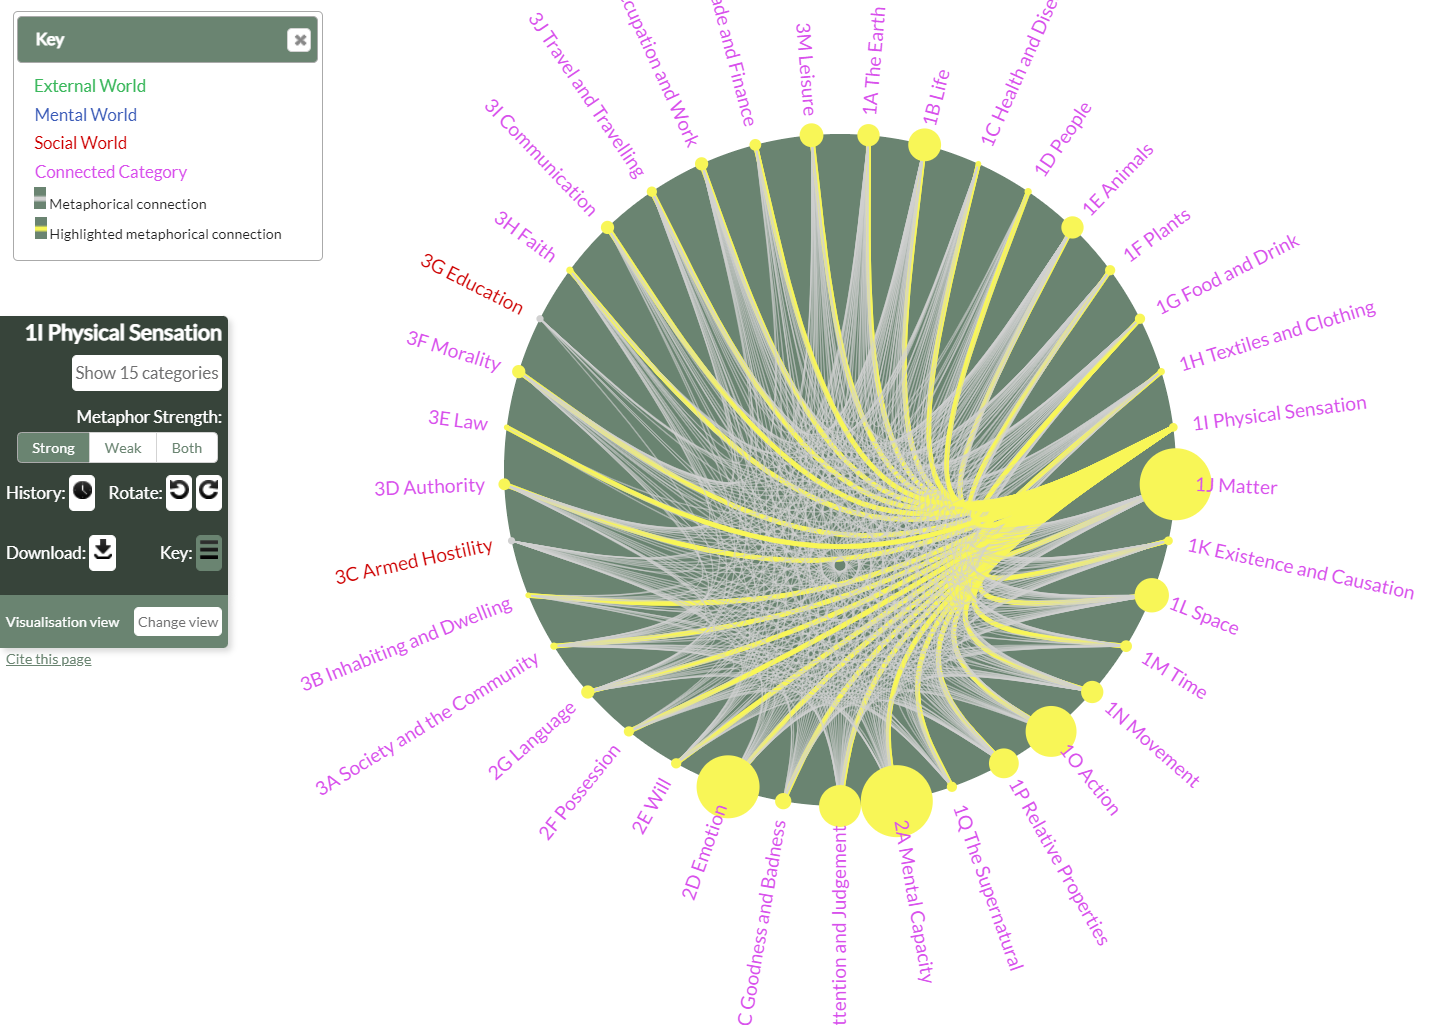
\includegraphics{introduction/fig/MappingMetaphor.png}
	}
	\caption[]{\label{fig:Introduction:MM} Screenshot of the \textit{Mapping Metaphor} website, which visualizes metaphorical connections between semantic fields.}
\end{figure}

% Piek Vossen:
%De relatie tussen de tekst en de figuur blijft vaag. De figuur is complex en het is niet duidelijk wat de bijdrage is aan het verhaal. Dit zoud je moeten uitleggen of de figuur wegalten.


Since lexicons are culture-specific, thesauri allow one to study a culture.\footnote{Kay and Roberts, \textit{The Encyclopedia of Language and Linguistics}, s.v. `Thesaurus'. An introduction to links between language and culture -- including vocabulary expansion owing to inventions and social attitudes reflected in expressions -- is provided by Kay and Allan, `Language and Culture'. Furthermore, Chapter 8 of the dissertation reflects on \textit{A Thesaurus of Old English}, specifically, and its relation to the culture of its early medieval speakers.} One manner in which important cultural aspects can be studied is by noting which words exist, or existed, in a vocabulary. In Old English, for instance, the lexical item \textit{wergild} denotes the legal value of a person's life.\footnote{Bosworth and Toller, \textit{An Anglo-Saxon Dictionary}, s.v. `wer-gild'.} The existence of this word, or perhaps rather the need for it, is a reflection of the fact that the penal laws of this early medieval society often required the perpetrator to recompense damages to other people by the amount of money the injured (or killed) person was deemed worth in society. The higher the rank of a person, the higher their worth.\footnote{Wormald, `Anglo-Saxon Society and its Literature', p. 11.} Further cultural insights can be gained from thesauri by analysing what distinctions people in a culture felt warranted reflection in their vocabulary. The group of loosely synonymous words for body in \textit{TOE}, for instance, includes the lexical items \textit{līc} and \textit{līchama}. The former generally referred to dead bodies; the latter to living --- a distinction early medieval English speakers felt necessary to maintain in order to express their thoughts.\footnote{Bosworth and Toller, \textit{An Anglo-Saxon Dictionary}, s.v. `líc' and `líc-hama'.}

Moreover, the importance of concepts in a culture can be judged by their elaboration in the available vocabulary: a relatively large number of words to express related notions and the nuances between them tends to convey such significance.\footnote{Wierzbicka, \textit{Understanding Cultures through their Key Words}, pp. 10–11.} In the surviving Old English vocabulary, for instance, the number of words to express bondage, slavery is quite sizeable, ``show[ing] how this warrior society was sustained by a class of unfree [...] men and women''.\footnote{Momma, Review of \textit{A Thesaurus of Old English}, p. 80.} Another striking example is that \textit{TOE} lists thirty-six Old English words for cloak-like garments. The great variety in words available to the Anglo-Saxons to describe these garments ``suggests that cloaks were a common garment, worn by different social classes''.\footnote{\textit{Learning with the Online} Thesaurus of Old English, section `Unit 5 Clothing'.}

Next to cultural research, thesauri are also of great value for literary-critical research. By annotating literary works with definitions in a lexicographic work, it is possible to indicate, per word, which specific meaning an author must have intended to convey. Cases of ambiguity can be made explicit by referencing multiple such definitions. Doing so may aid scholars in discussions on what the intentions and implications are of a literary work. Applying definitions from a thesaurus rather than from a dictionary has the advantage that scholars can, through the topical system of the thesaurus, obtain further insights into the diction and stylistic choices made by authors. Which lexical items were available to Shakespeare? Which ones seem to have been restricted to poetry (possibly because they were considered archaic), and do such restrictions appear to have had an impact on the word choices Shakespeare made for his plays? Which words did the poet and playwright prefer over others that expressed the same notion? In fact, answering questions on stylistic preference may help in establishing the author of a text.\footnote{An example of lexical evidence towards establishing the author of an anonymous text can be found in Bremmer, `Old English ``Cross'' Words'. In surveying Old English words denoting Christ's cross, Bremmer concludes that the word \textit{rōdehengen} must have been Ælfric of Eynsham's ``own coinage'' (p. 220) and strengthens the claim that the anonymous, liturgical text in which this word is found, too, is by the hand of this medieval abbot. A further exploration and analysis of Ælfric's lexical preferences, utilizing a thesaurus, can be found in Van Baalen, `Identifying, Categorising and Exploring ``Ælfrician'' Vocabulary'.} By applying statistical analyses, using thesauri to deduce which alternatives would have been available for a particular word, the deduced information on preferences could lead to establishing authorial fingerprints, as it were, which may assist in identifying which other literary works likely belong to the same author.\footnote{This approach is not unlike research done in the Lexomics programme (see `Lexomics'), although there no advantage is taken yet of thesauri for their knowledge on alternative phrasings that may have been available to a specific author.} 

In short, not only have thesauri proven themselves to be major assets in everyday use, they have been shown to be of great worth in various fields of research --- research not limited to linguistics, but extending to cultural, anthropological, and literary-critical research.


\section{Digital research opportunities}
\label{sect:Introduction:Impediments}

While most thesauri were fashioned to categorise contemporaneous vocabularies,\footnote{E.g., McArthur, \textit{Longman Lexicon of Contemporary English}; Wilkinson, \textit{Thesaurus of Traditional English Metaphors}.} very few have been fashioned with a historical language as their subject.\footnote{See Chapter 1.} %Even Latin, the scholarly language of the West during the Middle Ages, is yet to be captured in a comprehensive topical thesaurus.37 %As for diachronic topical thesauri, their number is exceptionally small. In fact, the Historical Thesaurus of English (HTE) has so far remained the only exception.38 The only other diachronic topical thesaurus that appears to be currently under development is the Thesaurus of Scots – an effort led by the same university as that behind HTE.39
The lack of such thesauri -- in spite of their abundant and diverse uses -- is straightforward to explain. Developing and publishing the first edition of \textit{TOE}, for instance, has taken a team of researchers over fifteen years.\footnote{Roberts, `Towards an Old English Thesaurus'.} \textit{HTE}, covering a vastly larger time period, has taken a team of two hundred thirty people well over forty years to develop.\footnote{These statistics can be found in the section `Stats and Figures' of \textit{HTE}. Unsurprising for such vast projects, the duration can partly be attributed to funding issues (Kay et al., `Unlocking the OED', p. xv).} These staggering numbers are certain to discourage most scholars from attempts at manually fashioning comprehensive thesauri of other historical languages. Future research would therefore benefit greatly from means to develop these resources in an automated manner and, arguably more important, to improve the dissemination form of existing thesauri in order to elaborate on and reuse the knowledge within. Such an improved dissemination may facilitate novel analyses and reuse of topical systems for other, related languages.\footnote{See the expand method as utilised by, for instance, Miháltz et al., `Methods and Results of the Hungarian WordNet Project'; and by Fernández-Montraveta et al., `The Spanish Version of WordNet 3.0'.} In fact, improving the form and method of dissemination of these thesauri should offer opportunities for novel research.

Reviews of \textit{TOE} foreground a number of opportunities for improving the dissemination of historical language thesauri.\footnote{The following reviews of \textit{TOE} have been consulted: Bremmer, Cavill, Conner, Dance, Görlach, Momma, Van Gelderen.} A prominent shortcoming of current editions is the inability to query and reuse the information contained in the thesauri in a way other than its editors had foreseen. The digital versions of \textit{TOE} and \textit{HTE} employ database-technology based on tabular storage of their data.\footnote{Both \textit{TOE} and \textit{HTE} employ MySQL database technology, as stated in the section `Creation of the \textit{Thesaurus}' of \textit{TOE}.} This data is subsequently shared, or rather visualised, in a searchable and browsable manner. However, this way of sharing proves to be rather limited. 
%To illustrate, lexical items on these websites cannot be referenced explicitly in a straightforward manner. through a Web address (or URL) and, as such, researchers will need to develop a custom system if they wish to communicate about these items specifically or to attach further knowledge.\footnote{} 
%Moreover, 
Users are unable to query or visualize these datasets in another manner than those provided for by the existing user interfaces of \textit{TOE} and \textit{HTE}. 

An example of a welcome query to be run against thesaurus content (a query that \textit{TOE} and \textit{HTE} currently do not allow) is one that provides statistics on the sizes of its semantic fields. As Anna Wierzbicka notes, important concepts in a society often witness cultural elaboration; that is, the availability of a relatively large number of words to express related notions and the nuances between them.\footnote{Wierzbicka, \textit{Understanding Cultures through their Key Words}, pp. 10–11.} Supplying users with such key statistics is straightforward within a digital environment, without them having to count the lexical items manually. %\footnote{I have implemented and demonstrated such functionality in previous research; see Stolk, `Welcoming the \textit{Thesaurus of Old English Statistics}'.}
For such functionality on statistics and other aspects to be added by parties other than the publisher, thesauri content should be reusable, in a storage format that does not favour one perspective (or query) over another.

Another area in which the dissemination of thesauri can be improved is in the availability of tagging information. In \textit{TOE}, for instance, indications of date and dialect are notably absent.\footnote{Bremmer, `Treasure Digging', p. 111; Görlach, Review of \textit{A Thesaurus of Old English}, p. 399; Dance, Review of \textit{A Thesaurus of Old English}, p. 313.} As it stands, all items are treated as belonging to ``a single geographically and temporally indistinguishable mass''.\footnote{Dance, Review of \textit{A Thesaurus of Old English}, p. 313.} Moreover, expanding thesauri with such information per lexical item will allow scholars to create subthesauri: thesauri filtered to display only those lexical items that meet a set of given criteria. For a diachronic thesaurus this could be a selection of a smaller time frame within the covered period. The editors of \textit{HTE}, for instance, point out that their thesaurus could be used to determine which lexical items will have been available to Shakespeare.\footnote{Kay et al., `Unlocking the OED', p. xiv.} However, the website does not allow the creation of a subthesaurus containing only those lexical items that were available during the life of Shakespeare --- or any other subthesaurus for that matter. Any filtering is left as exercise to the user. \textit{TOE}, too, includes valuable tagging information, stating whether its lexical items are found only in poetry or only in glosses. Although a previous, digital edition of \textit{TOE} allowed listing all lexical items tagged with a specific flag, the current edition no longer sports such helpful filtering capabilities.\footnote{For a description of the \textit{TOE} website previously available and its filtering on tagging information, see Stolk, `Welcoming the \textit{Thesaurus of Old English Statistics}', pp. 11–14.} The current digital versions of these thesauri do not facilitate researchers in extending existing content with further salient information and, based on available tags, in scrutinizing only those items deemed of interest to them. In essence, the desire for extra tagging information -- just like the need to reuse thesauri data in other projects -- boils down to the need for extendibility: allowing further information to be contributed, making it possible to form new queries over the combined information, and ensuring visualisations will convey the new insights acquired by the extensions.

In short, current forms of historical language thesauri limit their utilization. An attempt to resolve some of these issues, taking into account recent developments in information technology and improving on existing specifications for sharing linguistic information on the Semantic Web, should open up these lexicographic resources further for novel research.

% Ik mis hier nog het perspectief van linked open data waaraan een bijdrage geleverd kan worden vanuit historische thesauri. Zo zijn lemon specificaties niet ingericht op historische en dynamische lexicons. Je zou dus ook een vraag andersom kunnen formuleren. Hoe moeten linked open data specificaties worden aangepast om tegemoet te komen aan de wensen van gebruikers van historische thesauri.

% Voornaamste punt gaat over de aanpassingen die nodig zijn voor lemon om historische en dynamische lexicale informatie adequaat weer te geven. Dat mag je explicieter benoemen en problematiseren wat mij betreft.


\section{Research objective} \label{sect:Introduction:Objectives}

Historical language thesauri offer a number of uses beyond discovering available alternative phrasings, but, as explained in the previous section, opportunities exist to further their utilization for research. The main objective of my dissertation is to explore these opportunities and improve the use of these valuable lexicographic resources across various disciplines in academia. The result should enable a wider use of these thesauri for cultural, linguistic, anthropological, and literary-critical research.

\subsection{Research questions}

The main question of my research is formulated as follows:

\begin{quote}\normalsize
How can Web-based dissemination of thesauri of historical languages, and thesauri in general, be improved so as to answer to the research needs of scholars in various disciplines?\end{quote}

\noindent This overarching research question is covered by three sub questions on historical language thesauri:
\begin{enumerate}
    \item What are the main components found in these thesauri?
    \item What are the main features, or functionality, of these thesauri that are desired for research?
    \item What digital form should these thesauri be published in on the Web -- and what modifications to current specifications ought to be implemented for this purpose -- to support a wider use of historical language thesauri in academia?
\end{enumerate}

\noindent The questions above are addressed in Part I and II of the dissertation. The answers and hypotheses yielded are subsequently adopted and evaluated, in Part III, through their application to the historical language thesaurus \textit{TOE}. 



\section{Dissertation outline} \label{sect:Introduction:Methodology}

%This section introduces the research approach and methodology towards answering the research questions by providing an overview of the various chapters. 
This section provides an overview of the various chapters which, together, aim to answer the research questions. Besides the introduction and conclusion, the dissertation contains nine chapters -- i.e., three peer-reviewed papers, two peer-reviewed articles, and four original chapters -- that are spread across three Parts.\footnote{The dissertation contains references to code (of both software and data transformations) that has been developed and published as part of this research. An overview thereof is provided in the \hyperref[fm:sourcecode]{`List of source code'} in the back matter of the dissertation.} These chapters are discussed in terms of their position within the overall dissertation, their relation to the research questions, and their approach and most notable findings.


\subsection*{Part I. Historical Language Thesauri and their Characteristics}

Answering the main research question demands an understanding of what historical language thesauri are and what needs researchers have in accessing them. Part I of the dissertation consists of two original chapters, which provide insight into these matters through an overview of the characteristics of historical language thesauri.

\textit{Chapter 1} addresses research sub question 1: ``What are the main components found in historical language thesauri?'' This chapter draws from two types of sources in order to provide an overview of the information found in thesauri: (1) existing historical language thesauri of Scots and English and (2) publications and handbooks on both thesauri and lexicography in general. In the analysis and resulting overview, the focus lies on the knowledge contained within thesauri rather than at how that content is presented. Knowledge on the former can be used to produce multiple different presentations of the same thesaurus content, whilst the latter would mostly serve a single form of presentation and varies between different publications of a thesaurus (e.g., print editions and online editions). The three main parts of thesauri distinguished are: (1) the topical system, which is a hierarchy of semantic concepts; (2) lexical senses, which are words or phrases in a specific sense, positioned within the overarching topical system; and, optionally, (3) relations of synonymy, indicated through groupings of lexical senses.

\textit{Chapter 2} addresses research sub question 2: ``What are the main features, or functionality, of historical language thesauri that are desired for research?'' This chapter consults, in addition to the sources for Chapter 1, academic reviews of these thesauri and notable research employing them. These sources help establish which aspects of the existing historical language thesauri are deemed an asset, and which were found wanting or absent. Further input was gathered through a series of workshops surrounding a single thesaurus (\textit{TOE}) in order to obtain further research needs. The resulting information on desired functionality -- i.e., navigation, resource views, extension, analyses, and data management -- has been translated to a set of requirements for the digital form proposed for thesaurus publications on the Web and for the web application developed for interacting with these lexicographic resources.

% REQUIREMENTS EVOKE
%
%R1. Navigation.      / Browsing
%R2. Resource views.  / Browsing
%R3. Extension.  / Expansion
%R4. Analyses.   / Filtering & Querying
%R5. Data management.  / Reuse 
%
%AR1. Interoperable data form. / Filtering & Querying
%AR2. Decentralized data. / Reuse
%AR3. Support limited licenses. / Reuse



\subsection*{Part II. Historical Language Thesauri and a Digital Form on the Semantic Web}

Acknowledging the determined characteristics, both current and desired, of historical language thesauri, Part II explores a suitable digital form for their publication on the Web. These explorations are covered by one original chapter and two peer-reviewed publications.

\textit{Chapter 3} reflects on existing Web-based publications of historical language thesauri, discusses best practices for publishing data on the Web, and proposes a digital form for these thesauri that may be more appropriate for the research needs in mind than those of existing publications. The digital form proposed, which adopts Linked Data paradigms, facilitates data being FAIR (findable, accessible, interoperable, reusable). Through an analysis of each typical information component found in thesauri, a combination of suitable Linked Data data vocabularies is constructed and advocated in which to express thesauri. The combination and use of these vocabularies has, in a wider community towards standardization of the representation of linguistic and lexicographic resources on the Web, recently been termed Linguistic Linked Data.

The next two chapters are peer-reviewed papers published as part of conference proceedings, both of which offer findings on one of the core data vocabularies of Linguistic Linked Data, Lemon-OntoLex, and its applicability to thesauri. \textit{Chapter 4}, entitled `OntoLex and Onomasiological Ordering: Supporting Topical Thesauri', was published as part of the proceedings of the conference `Language, Data, and Knowledge 2017', Galway. This paper argues that Lemon-OntoLex is, on its own, insufficient for representing a large proportion of existing thesauri. After demonstrating the current expressivity and mentioned shortcoming of Lemon-OntoLex through two case studies (i.e., \textit{The Historical Thesaurus of the Oxford English Dictionary} and \textit{The Scots Thesaurus}), the paper proposes the addition of a relation to the OntoLex vocabulary: \texttt{ontolex:isSenseIn}. The findings and proposal of this paper was further discussed within the OntoLex community and resulted in the creation of a complementary data vocabulary, \textit{lemon-tree}, which is treated in the second paper included in the dissertation.\footnote{Based on feedback from the OntoLex community, the proposed \texttt{isSenseIn} was included in the \textit{lemon-tree} model as \texttt{isSenseInConcept}.}

\textit{Chapter 5}, a peer-reviewed paper entitled `\textit{lemon-tree}: Representing Topical Thesauri on the Semantic Web', was published as part of the conference proceedings of `Language, Data, and Knowledge 2019', Leipzig. 
%At the time of writing, lexicographic resources other than dictionaries had not been the main focus of efforts surrounding Linguistic Linked Data. 
This paper analyses fundamental needs for representing thesauri as Linguistic Linked Data and offers a solution for capturing two important aspects not covered by Lemon-OntoLex: (1) levels that can be distinguished in the topical system of thesauri and (2) a looser form of categorization than lexicalization. The necessary terminology for these aspects has been made available in an information model called \emph{lemon-tree}, facilitating publications of thesauri as Linguistic Linked Data.

\subsection*{Part III. Disseminating and Evaluating \textit{A Thesaurus of Old English} as Linguistic Linked Data}

The FAIR digital form of thesauri on the Web, proposed in Part II, is evaluated in Part III. Here, the case study of a single historical language thesaurus, \textit{TOE}, is discussed in-depth: its transformation to the digital form, dissemination through the novel web application Evoke, and utilization in research across various disciplines in academia. Thus, this part assesses to what extent Linguistic Linked Data, and the manner in which it is disseminated, allows for a wider use in academia than existing paper and digital editions of historical language thesauri. Part III contains three peer-reviewed publications and one original chapter. 

\textit{Chapter 6} is a paper, entitled `\emph{A Thesaurus of Old English} as Linguistic Linked Data: Using OntoLex, SKOS and \emph{lemon-tree} for Bringing Topical Thesauri to the Semantic Web', presented at `eLex 2019', Sintra. This paper discusses the process of porting \textit{TOE} to the Web-based form and provides recommendations for representing topical thesauri on the Web, whilst granting insights into aspects that may be encountered in porting similar lexicographic resources in the future. In order to support future work on other thesauri, the automated process created for porting this thesaurus has been made available via open access, too.\footnote{See \hyperref[fm:sourcecode]{`List of source code'} in the back matter of the dissertation.}

\textit{Chapter 7} is the article `Evoke: Exploring and Extending \textit{A Thesaurus of Old English} using a Linked Data Approach'. Published in the international peer-reviewed journal \textit{Amsterdamer Beiträge zur älteren
Germanistik} in 2021, this article details the web application Evoke. This web application, developed as part of this research, offers functionality for navigating, viewing, extending, and analysing thesaurus content that is represented as Linguistic Linked Data. Figure \ref{fig:Introduction:Evoke} illustrates the ability to navigate the topical system of a historical language thesaurus. So-called breadcrumbs indicate the current location in the topical system: starting from ``Power, might'' down to, currently in view, ``Freedom, being free''. The large pane in the user interface here indicates which subordinate categories, such as ``A free man'' and ``A free woman'', are available to the user for navigating further down the semantic hierarchy that the topical system constitutes. The functionality of Evoke, including the means to navigate, is founded on the research needs that surfaced in Part I of the dissertation and in various workshops referred to earlier. As the article demonstrates, Evoke proves to be a powerful research tool that facilitates its users to perform novel cultural linguistic analyses over multiple sources.

\begin{figure}[htb!]
	\resizebox{\textwidth}{!}{
		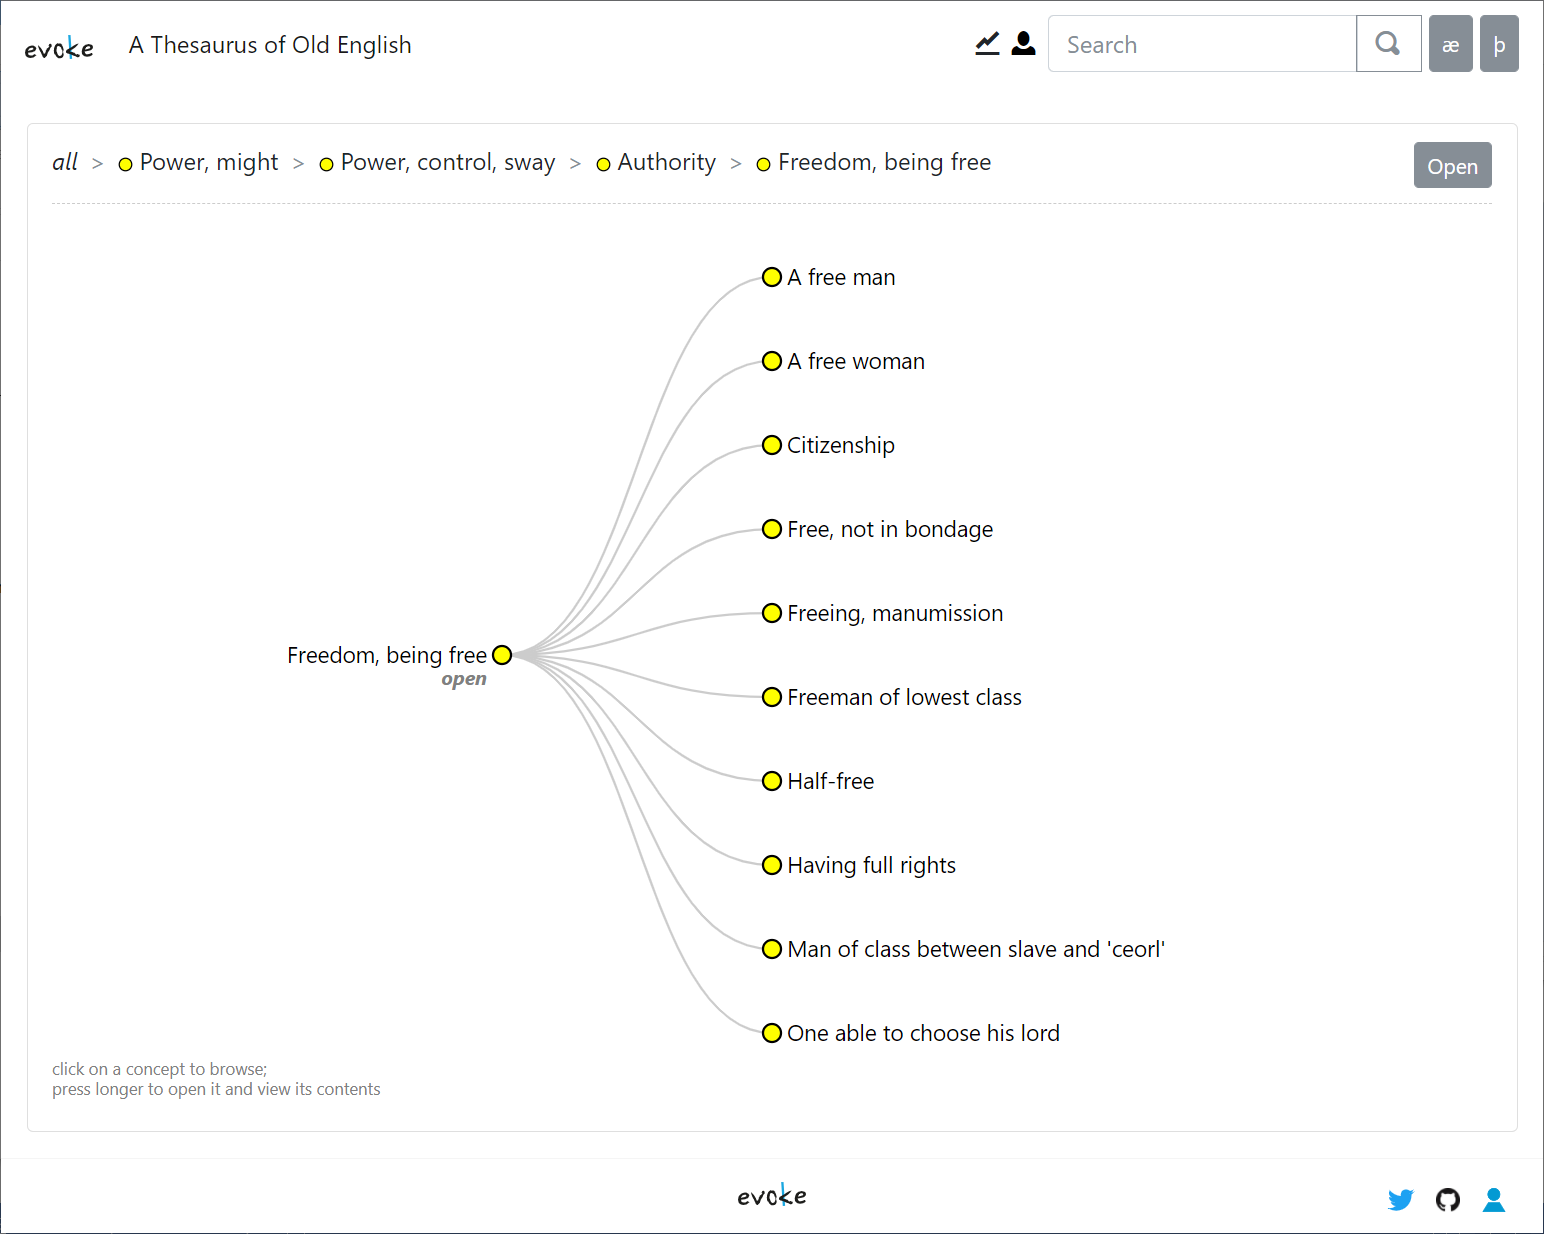
\includegraphics{introduction/fig/Evoke.png}
	}
	\caption[]{\label{fig:Introduction:Evoke} Navigating the topical system of \textit{TOE} in the web application Evoke.}
\end{figure}


\textit{Chapter 8}, following the chapter on Evoke, assesses the usefulness of the dissemination of \textit{TOE} as Linguistic Linked Data through the discussion of a number of research case studies. A collaborative project, titled `Exploring Early Medieval English Eloquence' (EEMEE), was established for this purpose. The project has brought together scholars from universities and lexicographic institutions from across Europe to explore -- and elaborate on -- the contents of \textit{TOE} using the web application Evoke. 
%Participating researchers (and in educational settings, their students) used Evoke to explore the contents of this thesaurus alongside additional material. 
Their case studies, the majority of which have been published as part of a special issue of the international, peer-reviewed journal \textit{Amsterdamer Beiträge zur älteren Germanistik}, are summarized in this chapter, along with reflections on the benefits and disadvantages of the new digital form and dissemination of the thesaurus concerned.

\textit{Chapter 9} is an article on one of the research case studies mentioned in Chapter 8, 
%here included in its entirety. 
%The article, 
co-written by Rita van de Poel and myself, %is
titled `A Case of Kinship: Onomasiological Explorations of \textsc{kinship} in Old Frisian and Old English'. Explorations of Old Frisian and Old English lexis in the semantic field of \textsc{kinship} are realized by connecting Old Frisian lexis to the overarching structure of \textit{TOE}. The resulting dataset for \textsc{kinship} in Old Frisian thus shares its semantic framework with that for Old English lexis. As the article demonstrates, this approach facilitates comparative analyses of the two historical languages, on an onomasiological level, which leads to new insights into linguistic and cultural aspects of these two languages and their language communities.

\vspace{\baselineskip}
%\subsection*{Conclusion}
\noindent
Lastly, the dissertation concludes by providing answers to the research questions, reflecting on the extent with which the proposed dissemination form of historical language thesauri overcomes the listed impediments for research, and discussing the potential future impact of the research presented here. %Since semantic field studies use the same building blocks as historical language thesauri... and similarities w/ other content attached to thesauri


\section{Related work}
\label{sect:Introduction:Related}

Digital approaches for investigating various facets surrounding language, including the structure of vocabularies and diachronic perspectives on language development, are by no means new.\footnote{This section draws on the overview of related work as published in Stolk, `Evoke'.} Such matters have often been explored, in various branches of computational linguistics, with digital corpora and analytical tools.\footnote{Sula and Hill, `The Early History of Digital Humanities'.} Onomasiological approaches are included amongst them, most notably through the use of thesauri and smaller semantic field studies.\footnote{\textit{HTE} lists many such studies in its `Bibliography' section.} Since the last century, research programmes have sought to further harness the potential of digital thesauri, whether digitized or born-digital. Automated uses, taking advantage of their digital form, include natural language processing and automated translations.\footnote{See, for instance, the use of machine-learning based on BERT in Kohli, `Transfer Learning and Augmentation for Word Sense Disambiguation'.} The next paragraphs will position my dissertation within a number of important developments within the field of Digital Humanities that deal with the study of lexicography and onomasiology.

The research in my dissertation shares its aim of increasing the availability of research infrastructure for language resources with recent European initiatives. Notable infrastructures for the Humanities are CLARIN (Common Language Resources and Technology Infrastructure)\footnote{De Jong et al., `Interoperability in an Infrastructure Enabling Multidisciplinary Research'.} and DARIAH (Digital Research Infrastructure for the Arts and Humanities)\footnote{Maryl et al., `Future of Scholarly Communication'}. These infrastructures allow researchers to work with, amongst others, textual corpora and natural language processing. Topical thesauri, the focus in this study, are not included in these two infrastructures. Indexing thesauri, however, are supported and are published as Linked Data.\footnote{`Vocabs Services', \textit{DARIAH}.} This format, which is also adopted in my dissertation, has been refined and standardized for linguistic resources in the Linguistic Linked Data community.\footnote{Cimiano et al., \textit{Linguistic Linked Data}.} In fact, CLARIN and the Linguistic Linked Data community seek to strengthen collaborations and have discussed common goals.\footnote{Stokman, `A Recap on the CLARIN Café on Linguistic Linked Data', \textit{CLARIN}.}

An important context for the research presented in the dissertation, as alluded to in the previous paragraph, is the efforts surrounding Linguistic Linked Data. As Declerck et al. have observed, these efforts play ``an increasing role in eLexicography''.\footnote{Declerck et al., `Recent Developments for the Linguistic Linked Open Data Infrastructure', p. 5664.} The English WordNet, for instance, has recently been ported to this model.\footnote{McCrae et al., `English WordNet 2020'.} Moreover, several recent initiatives aim at building and maintaining Linguistic Linked Data resources, including the H2020 projects ELEXIS (2018–22), Prêt-à-LLOD (2019–22) and the COST Action NexusLinguarum (2019–23).{\interfootnotelinepenalty=10000\footnote{ELEXIS: \url{https://cordis.europa.eu/project/id/731015}, 2018–2022; Prêt-à-LLOD: \url{https://cordis.europa.eu/project/id/825182}, 2019–2022; NexusLinguarum: \url{https://www.cost.eu/actions/CA18209}, 2019–2023.}} Tooling in these initiatives that work with Linguistic Linked Data focus on creation, discovery, transformation, and linking.\footnote{Declerck et al., `Recent Developments for the Linguistic Linked Open Data Infrastructure'.} Examples of such tools include LingHub, which offers discovery of language resources by searching through their metadata,\footnote{McCrae and Cimiano, `Linghub'.} and NAISC, used for aligning two RDF datasets. Unfortunately, most applications currently available for working with Linguistic Linked Data ``come with a considerable entry barrier and they address the advanced user of RDF technologies rather than a typical linguist''.\footnote{Chiarcos et al., `On the Linguistic Linked Open Data Infrastructure', p. 13.} The web application Evoke, developed as part of my dissertation, is amongst the first range of applications that aims to provide a user-friendly interface for such resources and to open them up to a wider audience. Other notable applications that provide user interfaces for Linguistic Linked Data resources are VocBench 3 and LexO.\footnote{Stellato et al., `VocBench 3'; Bellandi and Giovannetti, `Involving Lexicographers in the LLOD Cloud with LexO'.} Both of these web-based platforms allow users to edit and view Linguistic Linked Data in a user-friendly manner. However, unlike Evoke, they lack functionality to perform onomasiological analyses: their main aim is to manage and publish content collaboratively.

Lastly, a number of recent research programmes have increased efforts that expand the use of thesauri to other domains. The onomasiological lens that \textit{HTE} provides, for instance, has been utilized for mapping metaphors throughout the history of the English language and for semantically annotating entire textual corpora for topical analyses.\footnote{\textit{Mapping English Metaphor through Time}; Piao et al., `A Time-sensitive Historical Thesaurus-based Semantic Tagger for Deep Semantic Annotation'.} Similarly, my dissertation seeks to contribute novel methods to Digital Humanities research for engaging with thesauri. By offering statistical analyses utilizing the semantic hierarchy of these lexicographic resources, and by allowing researchers to link additional information to thesaurus content, the web application Evoke grants new, meaningful insights into a language and the use of its vocabulary in cultural expressions (e.g., individual texts or entire oeuvres). As Chapter 8 demonstrates, the functionality available offers results that provide additional knowledge, but may also raise new questions that warrant a closer inspection of the cultural context (e.g., textual, historical, socio-economic). The research presented here, therefore, is firmly rooted in Digital Humanities, and provides the means to explore Humanities-based questions through digital resources that complement 
%, but not supplant, 
knowledge and expertise of scholars.


%\section{Valorisation of knowledge}
%Although the proposed research is situated within digital humanities, the academic field where humanities and the electronic environment meet, the results will have practical uses beyond an academic setting. Indeed, although the scope of my thesis focuses on thesauri on historical periods, the results will also be functional – and valuable – for non-historical content. As many organisations are looking into ways to express their vocabularies and to share their concepts with other parties, a streamlined process to fashion topical thesauri and to share and extend their contents afterwards is a welcome one. Such thesauri can improve clarity of meaning for these organisations both internally and externally. To illustrate, one can imagine that it would be wise to avoid ambiguities in reports when it comes to pointing out deficient aspects of a particular road. The Dutch vocabulary, however, contains a particular word that may lead to exactly such ambiguity: kunstwerk. The word, which in everyday language refers to a piece of art, carries the meaning of an artificial, man-made construction in the engineering sector.55 Considering roundabouts were not uncommonly decorated with a piece of art at their centre in the Netherlands, statements that the kunstwerk of a particular roundabout was deficient could refer to either such a piece of art or the very road of the roundabout itself.56 Misinterpretations can be avoided by referring to concept definitions clarified in a topical thesaurus. The position of one meaning for kunstwerk can be placed in one context or position in the thesaurus, and the other meaning in another. 
%
%Another example, in this case from the academic world, that could benefit from elucidation by means of a thesaurus is the word professor. This word has various meanings in universities across the world – even within a single language – ranging from an academic who is responsible for the development of and education on their field of expertise to any person who acts as tutor at a university.57 By referring to the intended meanings in a topical thesaurus, in which it is apparent which meanings of this word are more specific or more general than others, the nuances between these definitions can be portrayed better and misunderstandings in communication can be avoided. 
%
%Thesauri that are multilingual or include multiple contexts can be of great value not only to indicate the intended meaning of word, but also to aid translations. One such possible thesaurus would be one containing academic positions as they are known throughout the world, making it possible to translate the word professor from one context, with a specific meaning, to the term used for that very meaning in a second context. A prime example of a topical thesaurus already in use to position concepts in their appropriate contexts is EuroVoc, a multilingual thesaurus that covers the activities of the European Union. This thesaurus is in use with a number of European bodies (including the European Parliament).58 In addition, utilisation of topical thesauri has allowed a number of organisations to categorise reports and automate their further processing to a high degree, again foregrounding the practical importance of these semantic treasure troves.59



\section*{References}

\begin{list}{}%
{\leftmargin=0.5in \itemindent=-0.5in}
\setlength{\itemsep}{0pt}
\setlength{\parskip}{0pt}
\setlength{\parsep}{0pt}

%\item 
%\textit{A Companion to the Latin Language}, ed. J. Clackson, \textit{Blackwell Companions to the Ancient World} 132 (Oxford, 2011).

%\item
%\textit{A Thesaurus of Old English}, eds. J. Roberts and C. Kay with L. Grundy. \url{https://oldenglishthesaurus.arts.gla.ac.uk/}. Accessed: 15 March 2022.


\item % CITED IN CHAPTER
Adamska-Salaciak, A., Review of \textit{Historical Thesaurus of the Oxford English Dictionary} by C. Kay et al., \textit{International Journal of Lexicography} 23.2 (2010), 227–33.

%\item
%Alexander, M. G., `Historical Thesaurus of English Online'. \textit{The Linguist List} 26.819 (2015).

\item % CITED IN CHAPTER
Allan, K., \textit{Metaphor and Metonymy: A Diachronic Approach}, Publications of the Philological Society 42 (Malden, 2008).

%\item
%Allemang, D. and J. Hendler, \textit{Semantic Web for the Working Ontologist: Effective Modeling in RDFS and OWL}, 2nd edn (Waltham, 2011).

%\item
%Beekmans, M. and M. Zebracki, `Rotondekunst met een kwinkslag', Rooilijn: Tijdschrift voor Wetenschap en Beleid in de Ruimtelijke Ordening 47.1 (2014): 16–21.

\item % CITED IN CHAPTER
Bellandi, A. and E. Giovannetti, `Involving Lexicographers in the LLOD Cloud with LexO, an Easy-to-Use Editor of Lemon Lexical Resources', Proceedings of the 7th Workshop on Linked Data in Linguistics (2020), 70–4. \url{https://aclanthology.org/2020.ldl-1.10.pdf}.

%\item
%Berners-Lee, T. et al., `The Semantic Web', \textit{Scientific American Magazine} (May 2001).

%\item
%Berners-Lee, T., \textit{Linked Data: Design Issues}. \url{https://www.w3.org/DesignIssues/LinkedData.html}. Last updated: 18 June 2009. Accessed: 18 January 2016.

\item % CITED IN CHAPTER
Bosworth, J. and T. N. Toller, \textit{An Anglo-Saxon Dictionary Based on the Manuscript Collections of the Late Joseph Bosworth} (London, 1898), \textit{Supplement by T. N. Toller} (Oxford, 1921), \textit{with Enlarged Addenda and Corrigenda by A. Campbell} (Oxford, 1972).

\item % CITED IN CHAPTER
Bremmer Jr, R. H., `Treasure Digging in the Old English Lexicon', Review of \textit{A Thesaurus of Old English} by J. Roberts et al., \textit{NOWELE} 40 (2002), 109–14.

%\item
%Bremmer Jr, R. H., \textit{An Introduction to Old Frisian: History, Grammar, Reader, Glossary} (Amsterdam, 2009).

\item % CITED IN CHAPTER
% book chapter, West Virginia University Press
Bremmer Jr, R. H., `Old English ``Cross'' Words', \textit{Cross and Cruciform in the Anglo-Saxon World: Studies to Honor the Memory of Timothy Reuter}, Medieval European Studies XI (Morgantown, 2010), 204-32.
%Bremmer Jr Rolf H. (2010), Old English "Cross" Words. In: Keefer S.L, Jolly K.L., Karkov C.E. (Eds.) Cross and Cruciform in the Anglo-Saxon World. Studies to Honor the Memory of Timothy Reuter. Morgantown, WV: West Virginia University Press. 204-232.

%\item
%Brinton, L. J., \textit{The Structure of Modern English: A Linguistic Introduction} (Amsterdam, 2000).

\item % CITED IN CHAPTER
Brewer, C., Review of \textit{Historical Thesaurus of the Oxford English Dictionary} by C. Kay et al., \textit{Review of English Studies} 61.252 (2010), 801–5.

\item % CITED IN CHAPTER
Busse, B., `A Celebration of Words and Ideas: The Stylistic Potential of the \textit{Historical Thesaurus of the Oxford English Dictionary}', \textit{Language and Literature} 21.1 (2012), 84–92. 

\item % CITED IN CHAPTER
Cavill, P., `Names and Things in Anglo-Saxon and Early Norman England', Review of \textit{A Thesaurus of Old English} by J. Roberts et al. and \textit{Words, Names and History: Selected Writings of Cecily Clark} by P. Jackson, \textit{Nottingham Medieval Studies} 41 (1997), 186–91.

\item % CITED IN CHAPTER
Celen, K. M. and Ş. Yalçin, `The Effects of Vocabulary Resource Use on Lexical Richness in L2 Writing', \textit{Milli Eğitim Dergisi} 50.230 (2021), 1039-58. doi: \href{https://doi.org/10.37669/milliegitim.687806}{\url{10.37669/milliegitim.687806}}.

\item % CITED IN CHAPTER
Chiarcos, C. et al., `On the Linguistic Linked Open Data Infrastructure', Proceedings of the 1st International Workshop on Language Technology Platforms (2020), 8–15. \url{https://www.aclweb.org/anthology/2020.iwltp-1.2}.

\item % CITED IN CHAPTER
Cimiano, P. et al., \textit{Linguistic Linked Data: Representation, Generation and Applications} (2020). doi: \href{https://doi.org/10.1007/978-3-030-30225-2}{\url{10.1007/978-3-030-30225-2}}.

%\item
%Clark Hall, J. R., \textit{A Concise Anglo-Saxon Dictionary}, 4th edn, \textit{with a Supplement by H. D. Meritt} (Cambridge, 1960).

\item % CITED IN CHAPTER
Coleman, J., \textit{Love, Sex and Marriage: A Historical Thesaurus}, Costerus New Series 118 (Amsterdam, 1999).

\item % CITED IN CHAPTER
Coleman, J., Review of \textit{Historical Thesaurus of the Oxford English Dictionary} by C. Kay et al., \textit{Word Structure} 6.2 (2013), 201–13.

\item  % CITED IN CHAPTER
\textit{Collins English Thesaurus}, eds. J. Crozier et al. (Glasgow, 2011). % eds. J. Crozier, L. Gilmour, and H. Hucker

\item % CITED IN CHAPTER
Conner, P. W., Review of \textit{A Thesaurus of Old English} by J. Roberts et al., \textit{Speculum} 73.3 (1998), 887–9.

\item % CITED IN CHAPTER
Crystal, D., \textit{Words in Time and Place: Exploring Language through the Historical Thesaurus of the} Oxford English Dictionary (Oxford, 2014).

\item % CITED IN CHAPTER
Dance, R., Review of \textit{A Thesaurus of Old English} by J. Roberts et al., \textit{Medium Ævum} 66.2 (1997), 312–3.

%\item
%Dallachy, F. and M. Alexander, `Versions and Conversions in the Historical Thesaurus of English', \textit{Mapping Metaphor with the} Historical Thesaurus. \url{http://blogs.arts.gla.ac.uk/metaphor/?p=273}. Blog. Last updated: 23 March 2015. Accessed: 16 January 2016. 

\item % CITED IN CHAPTER
Declerck, T. et al., `Recent Developments for the Linguistic Linked Open Data Infrastructure', Proceedings of the 12th Language Resources and Evaluation Conference (2020), 5660–7. \url{https://www.aclweb.org/anthology/2020.lrec-1.695}.

\item % CITED IN CHAPTER
De Jong, F. et al., `Interoperability in an Infrastructure Enabling Multidisciplinary Research: The case of CLARIN', Proceedings of the 12th International Conference on Language Resources and Evaluation (2020). \url{https://www.aclweb.org/anthology/2020.lrec-1.417/}.

\item % CITED IN CHAPTER
Diller, H., `Emotions in the English Lexicon: A Historical Study of a Lexical Field', \textit{English Historical Linguistics} 1992: Papers from the 7th International Conference on English Historical Linguistics, eds. F. Fernandez et al., Current Issues in Linguistic Theory 113 (Amsterdam, 1994), 219–34.

%\item
%Drout, M. D. C. et al., `Of Dendrogrammatology: Lexomic Methods for Analyzing Relationships among Old English Poems', \textit{JEGP} 110.3 (2011), 301–36.

\item % CITED IN CHAPTER
\textit{Encyclopedia of Language \& Linguistics}, 2nd edn, ed. K. Brown, 14 vols. (Oxford, 2006).

\item % CITED IN CHAPTER
`EuroVoc', \textit{EUR-Lex}. \url{https://eur-lex.europa.eu/browse/eurovoc.html}. Accessed: 15 March 2022.

\item % CITED IN CHAPTER
Faria, F., `Georges Cuvier et le premier paradigme de la paléontologie', \textit{Revue de Paléobiologie} 32.2 (2013), 297–302.

\item % CITED IN CHAPTER
Fernández-Montraveta, A., G. Vázquez, and C. Fellbaum, `The Spanish Version of WordNet 3.0', Text resources and Lexical Knowledge', \textit{Text, Translation, Computational Processing} (Berlin, 2008), 175–82.

%\item
%`Gemeenschappelijke Thesaurus Audiovisuele Archieven', \textit{Beeld en Geluid}.  \url{http://gtaa.beeldengeluid.nl/}. Accessed: 24 January 2016.

\item % CITED IN CHAPTER
Gánem-Gutiérrez, G. A. and A. Gilmore, `A Mixed Methods Case Study on the Use and Impact of Web-based Lexicographic Tools on L2 Writing', \textit{Computer Assisted Language Learning} 2021. doi: \href{https://doi.org/10.1080/09588221.2021.1987273}{\url{10.1080/09588221.2021.1987273}}.

\item % CITED IN CHAPTER
Görlach, M., Review of \textit{A Thesaurus of Old English} by J. Roberts et al., \textit{Anglia} 116.3 (1998), 398–401.

%\item
%Görlach, M., Review of \textit{Historical Thesaurus of the Oxford English Dictionary} by C. Kay et al., \textit{English Language and Linguistics} 15 (2011), 193–7.

%\item
%Hannam, J., \textit{God's Philosophers: How the Medieval World Laid the Foundations of Modern Science} (London, 2009).

%\item
%\textit{Historical Thesaurus of Scots}, ed. S. Rennie. \url{http://scotsthesaurus.org/}. Accessed 17 January 2016.

%\item
%Hofmann, D. and A. T. Popkema, \textit{Altfriesisches Handwörterbuch, unter Mitwirkung von G. Hofmann} (Heidelberg, 2008).

%\item
%Hollink, L. et al., `Thesaurus Enrichment for Query Expansion in Audiovisual Archives', \textit{Multimedia Tools and Applications} 49.1 (2010), 235–57. 

%\item
%Hristea, F., `On the Semiautomatic Generation of WordNet Type Synsets and Clusters', \textit{Journal of Universal Computer Science} 8.12 (2002), 1047–64.

\item % CITED IN CHAPTER
\textit{HTE} = \textit{The Historical Thesaurus of English}, eds. C. Kay et al. \url{https://ht.ac.uk/}. Accessed: 15 March 2022.

\item % CITED IN CHAPTER
Hüllen, W., \textit{A History of Roget's} Thesaurus\textit{: Origins, Development, and Design} (Oxford, 2005).

%\item
%Ilson, R. F., `On the Historical Thesaurus of the Oxford English Dictionary', \textit{International Journal of Lexicography} 24.2 (2011), 241–260.

%\item
%`Integrated Public Sector Vocabulary', \textit{Local Government Association}. \url{http://id.esd.org.uk/list/subjects}. Accessed: 24 January 2016.

%\item
%Jarmasz, M. and S. Szpakowicz, `\textit{Roget's Thesaurus} and semantic similarity', Recent Advances in Natural Language Processing III: Selected Papers from RANLP 2003, eds. N. Nicolov et al., Current Issues in Linguistic Theory 260, 111–20 (Amsterdam, 2004).

%\item
%Kaltenbock, M. and E. Kruizinga, `Climate Technology Transfer Supported through Linked Data', Symposium Linked Data NL, Hilversum, 29 September 2015. Talk.

\item % CITED IN CHAPTER
Kay, C. and I. Wotherspoon, `Wreak, Wrack, Rack, and (W)ruin: The History of Some Confused Spellings', in Sounds, Words, Texts and Change: Selected Papers from 11 ICEHL, Santiago de Compostela, 7-11 September 2000, 129-43 (Amsterdam, 2002).

\item % CITED IN CHAPTER
Kay, C. and K. Allan, `Language and Culture', in \textit{English Historical Semantics}, Edinburgh Textbooks on the English Language - Advanced (Edinburgh, 2015).

\item % CITED IN CHAPTER
Kay, C. and M. Alexander, `Diachronic and Synchronic Thesauruses'. \textit{The Oxford Handbook of Lexicography} (Oxford, 2016), 367–80.

\item
Kay, C. et al., \textit{Historical Thesaurus of the Oxford English Dictionary} (Oxford, 2009).

\item % CITED IN CHAPTER
Kay, C. et al., `Unlocking the \textit{OED}: The Story of the \textit{Historical Thesaurus of the OED}', \textit{Historical Thesaurus of the Oxford English Dictionary}, eds. C. Kay et al. (Oxford, 2009), xiii–xx.

%\item
%Köbler, G., \textit{Altfriesisches Wörterbuch} (2014). \url{http://www.koeblergerhard.de/afrieswbhinw.html}. Accessed: 1 February 2016.

\item % CITED IN CHAPTER, online conference
Kohli, H., `Transfer Learning and Augmentation for Word Sense Disambiguation', Proceedings of the 43rd European Conference on Information Retrieval (2021), 303–11. doi: \href{https://dx.doi.org/10.1007/978-3-030-72240-1_29}{\url{10.1007/978-3-030-72240-1_29}}.

%\item
%`Language Acquisition 2: From Scratch to Print (2015--16)', \textit{University Leiden e-Prospectus}. \url{https://studiegids.universiteitleiden.nl/en/courses/49721/language-acquisition-2-from-scratch-to-print}. Accessed: 15 March 2022. 

\item % CITED IN CHAPTER
\textit{Learning with the Online Thesaurus of Old English}, eds. C. Hough and C. Kay. \url{https://oldenglishteaching.arts.gla.ac.uk}. Accessed: 15 March 2022.

%\item
%Lee, S. et al., `Automatic Generation of Concept Hierarchies using WordNet', \textit{Expert Systems with Applications} 35 (2008), 1132–44. 

%\item
%`Leiden, Delft and Erasmus to Apply ``Big Data'' for Urban Issues', \textit{Leiden University}. \url{https://www.universiteitleiden.nl/en/news/2016/02/leiden-delft-and-erasmus-to-apply-big-data-for-urban-issues}. News. Last updated: 9 February 2016. Accessed: 21 February 2016.

\item % CITED IN CHAPTER
`Lexomics', \textit{Wheaton College}. \url{http://wheatoncollege.edu/lexomics/}. Accessed: 22 February 2016.

%\item
%Loo, S., \textit{Legislative Indexing Vocabulary: The CRS Thesaurus} (Washington, 1998).

\item % CITED IN CHAPTER
\textit{Mapping English Metaphor through Time}, eds. W. Anderson, E. Bramwell, and C. Hough, (Oxford, 2016).

\item % CITED IN CHAPTER
\textit{Mapping Metaphor}. \url{http://mappingmetaphor.arts.gla.ac.uk/}. Accessed: 15 March 2022.

\item % CITED IN CHAPTER
Maryl, M. et al., `Future of Scholarly Communication: Forging an Inclusive and Innovative Research Infrastructure for Scholarly Communication in the Social Sciences and Humanities', Research Report, OPERAS (2021).

\item % CITED IN CHAPTER
McArthur, T., \textit{Longman Lexicon of Contemporary English} (Harlow, 1981).

\item % CITED IN CHAPTER
McCrae, J. et al., `English WordNet 2020', Proceedings of the Multimodal Wordnets Workshop at LREC 2020 (2020), 14–19.

\item % CITED IN CHAPTER
McCrae, J. and P. Cimiano, `Linghub: A Linked Data Based Portal Supporting the Discovery of Language Resources', Proceedings of the Posters and Demos Track of 11th International Conference on Semantic Systems (Vienna: 2015), 88–91. \url{http://dblp.uni-trier.de/db/conf/i-semantics/semantics2015p.html#McCraeC15}.

\item % CITED IN CHAPTER
`Medical Subject Headings RDF', \textit{U.S. National Library of Medicine}. \url{https://id.nlm.nih.gov/mesh/}. Accessed: 15 March 2022. 

\item % CITED IN CHAPTER
Miháltz, M. et al., `Methods and Results of the Hungarian WordNet Project', Proceedings of the 4th Global WordNet Conference (Szeged, Hungary, 2008), 311–20.

\item % CITED IN CHAPTER
Momma, H., Review of \textit{A Thesaurus of Old English} by J. Roberts et al., \textit{Notes and Queries} 50.1 (2003), 79–80.

\item % CITED IN CHAPTER
NAISC. \url{https://github.com/insight-centre/naisc}. Accessed: 15 March 2022.

\item
`NASA Thesaurus', \textit{Data.gov}. \url{https://catalog.data.gov/dataset/nasa-thesaurus}. Last updated: 12 November 2020.

%\item
%Navigli, R., `Word Sense Disambiguation: A Survey', \textit{ACM Computing Surveys} 41.2 (2009), 1–69.

%\item
%`OTL Library 1.7.1', \textit{Rijkswaterstaat}. \url{https://otl.rws.nl}. Accessed: 22 February 2016.


%\item
%`OWL 2 Web Ontology Language: Structural Specification and Functional-Style Syntax', 2nd edn, eds. B. Motik et al., \textit{W3C}. \url{https://www.w3.org/TR/owl2-syntax/}. W3C Recommendation. Created: 27 October 2009. Accessed: 18 January 2016.

\item % CITED IN CHAPTER
\textit{Oxford English Dictionary}. \url{https://www.oed.com}. Accessed: 15 March 2022.

\item % CITED IN CHAPTER
Piao, S. et al., `A Time-sensitive Historical Thesaurus-based Semantic Tagger for Deep Semantic Annotation', \textit{Computer Speech and Language} 46 (2017), 113–35.

%\item
%Piasecki, M. et al., `The WordNet Weaver: Multi-criteria Voting for Semi-automatic Extension of a Wordnet', in \textit{Advances in Artificial Intelligence}, eds. Y. Gao and N. Japkowicz. Lecture Notes in Computer Science 5549 (Berlin, 2009), 237–40.

%\item
%`RDF 1.1 Concepts and Abstract Syntax', eds. R. Cyganiak et al., \textit{W3C}. \url{https://www.w3.org/TR/rdf11-concepts/}. W3C Recommendation. Created: 25 February 2014. Accessed: 18 January 2016.

%\item
%`RDF 1.1 Semantics', eds. P. J. Hayes and P. F. Patel-Schneider, \textit{W3C}. https://www.w3.org/TR/rdf11-mt/. W3C Recommendation. Created: 25 February 2014. Accessed: 18 January 2016.

%\item
%`RDF Schema 1.1', W3C, eds. D. Brickley et al. https://www.w3.org/TR/rdf-schema/. W3C Recommendation. Created: 25 February 2014. Accessed: 18 January 2016.

%\item
%`RDF/OWL Representation of WordNet', eds. M. van Assem et al., \textit{W3C}. \url{http://www.w3.org/TR/wordnet-rdf/}. Last updated: 19 June 2006. Accessed: 15 March 2022.

\item % CITED IN CHAPTER
Roberts, J., `Towards an Old English Thesaurus', \textit{Poetica} 9 (1978), 56–72.

\item % CITED IN CHAPTER
Roberts, J., `\textit{A Thesaurus of Old English}: The Pilot Study for the Glasgow \textit{Historical Thesaurus}', \textit{Amsterdamer Beiträge zur älteren Germanistik} 81.3-4 (2021), 297–317. doi: \href{https://doi.org/10.1163/18756719-12340234}{\url{10.1163/18756719-12340234}}.

\item % CITED IN CHAPTER
\textit{Roget's} = Roget, P. M., \textit{Thesaurus of English Words and Phrases, Classified and Arranged so as to Facilitate the Expression of Ideas and Assist in Literary Composition} (London, 1852).

\item % CITED IN CHAPTER
Schendl, H., \textit{Historical Linguistics, Oxford Introductions to Language Study} (Oxford, 2001). 

%\item
%`Semantic Web', \textit{W3C}. \url{https://www.w3.org/standards/semanticweb/}. Accessed: 18 January 2016.

%\item
%Spevack, M., \textit{A Shakespeare Thesaurus} (Hildesheim, 1993).

\item`% CITED IN CHAPTER
Stellato, A. et al., `VocBench 3: A Collaborative Semantic Web Editor for Ontologies, Thesauri and Lexicons', \textit{Semantic Web} 11.5 (2020), 855–81.

\item % CITED IN CHAPTER
Stolk, S., `Welcoming the \textit{Thesaurus of Old English Statistics}: The \textit{Thesaurus of Old English} and the Vocabulary of Greetings', M.A. dissertation, Leiden University (2013). 

\item % CITED IN CHAPTER (or rather, mentioned)
Stolk, S., `OntoLex and Onomasiological Ordering: Supporting Topical Thesauri', Proceedings of the Linked Data Knowledge 2017 Workshops, NUI Galway, 18 June 2017, pp. 60–7. \url{http://ceur-ws.org/Vol-1899/OntoLex_2017_paper_3.pdf}.

\item % CITED IN CHAPTER (or rather, mentioned)
Stolk, S., `\textit{lemon-tree}: Representing Topical Thesauri on the Semantic Web', Proceedings of Linked Data Knowledge 2019, Leipzig, 20–23 May 2019. doi: \href{https://doi.org/10.4230/OASIcs.LDK.2019.16}{\url{10.4230/OASIcs.LDK.2019.16}}.

\item % CITED IN CHAPTER (or rather, mentioned)
Stolk, S., `\textit{A Thesaurus of Old English} as Linguistic Linked Data', Proceedings of eLex2019, Sintra, 1–3 October 2019. \url{https://elex.link/elex2019/wp-content/uploads/2019/09/eLex_2019_13.pdf}.

\item % CITED IN CHAPTER
Stolk, S., `Evoke: Exploring and Extending \textit{A Thesaurus of Old English} using a Linked Data Approach', \textit{Amsterdamer Beiträge zur älteren Germanistik} 81.3-4 (2021), 318–58. doi: \href{https://doi.org/10.1163/18756719-12340235}{\url{10.1163/18756719-12340235}}.

\item % CITED IN CHAPTER
Stokman, L., `A Recap on the CLARIN Café on Linguistic Linked Data', \textit{CLARIN}. \url{https://www.clarin.eu/news/recap-clarin-cafe-linguistic-linked-data}. Last updated: 17 May 2021.

\item % CITED IN CHAPTER
Sula, C. A. and H. V. Hill, `The Early History of Digital Humanities: An Analysis of Computers and the Humanities (1966–2004) and Literary and Linguistic Computing (1986–2004)', \textit{Digital Scholarship in the Humanities} 34 (2019), i190–206. doi: \href{https://doi.org/10.1093/llc/fqz072}{\url{10.1093/llc/fqz072}}.

\item % CITED IN CHAPTER
Tejada-Caller, P., `On \textit{Shapelings} and \textit{Childlings}: A Linguistic Approach to the Emergence of New Cultural Borders Between the Unborn and the New-born Child in EME (1500-1700)', \textit{Journal of English Studies} 18 (2020), 227-51. doi: \href{https://doi.org/10.18172/jes.4502}{\url{10.18172/jes.4502}}.

\item
\textit{Thesaurus Linguae Latinae}, ed. M. Hillen. \url{https://thesaurus.badw.de/en/}. Accessed: 15 March 2022.

\item % CITED IN CHAPTER
\textit{The Encyclopedia of Language and Linguistics}, ed. R. E. Asher, 10 vols. (Oxford, 1994).

\item % CITED IN CHAPTER
\textit{The Scots Thesaurus}, eds. I. Macleod et al. (Aberdeen, 1990).

\item % CITED IN CHAPTER
\textit{TOE} = \textit{A Thesaurus of Old English}, eds. J. Roberts et al. (Glasgow, 2015). \url{http://oldenglishthesaurus.arts.gla.ac.uk}. Accessed: 15 March 2022.

\item % CITED IN CHAPTER
Van Baalen, A., `Identifying, Categorising and Exploring ``Ælfrician'' Vocabulary Using the \textit{Dictionary of Old English}, \textit{A Thesaurus of Old English} and Evoke', \textit{Amsterdamer Beiträge zur älteren Germanistik} 81.3-4 (2021), 384–441. doi: \href{https://doi.org/10.1163/18756719-12340237}{\url{10.1163/18756719-12340237}}.

\item % CITED IN CHAPTER (or rather, mentioned)
Van de Poel, R. and S. Stolk, `A Case of Kinship: Onomasiological Explorations of \textsc{kinship} in Old Frisian and Old English', \textit{Amsterdamer Beiträge zur älteren Germanistik} 81.3-4 (2021), 457–92. doi: \href{https://doi.org/10.1163/18756719-12340239}{\url{10.1163/18756719-12340239}}.

\item % CITED IN CHAPTER
Van Gelderen, E., Review of \textit{A Thesaurus of Old English} by J. Roberts et al., \textit{Studies in Language} 27.1 (2003), 200–3.

\item % CITED IN CHAPTER
`Vocabs Services', \textit{DARIAH}. \url{https://www.dariah.eu/tools-services/tools-and-services/tools/vocabs-services/}.

\item % CITED IN CHAPTER
Wierzbicka, A., \textit{Understanding Cultures through their Key Words: English, Russian, Polish, German, and Japanese}, Oxford Studies in Anthropological Linguistics 8, ed. W. Bright (Oxford, 1997).

\item % CITED IN CHAPTER
Wilkinson, P. R., \textit{Thesaurus of Traditional English Metaphors}, 2nd edn (London, 2002). 

%\item
%\textit{WordNet: A lexical database for English}. \url{https://wordnet.princeton.edu/}.

%\item
%\textit{WordNet 3.0 in RDF}, eds. M. van Assem and J. van Ossenbruggen. \url{http://semanticweb.cs.vu.nl/lod/wn30/}. Last updated: 25 September 2010. Accessed: 17 January 2016.

\item % CITED IN CHAPTER
Wormald, P., `Anglo-Saxon Society and its Literature', \textit{The Cambridge Companion to Old English Literature}, eds. M. Godden and M. Lapidge (Cambridge, 1991), 1–22.

\end{list}